\section{Hardware}
\label{sec:hardware}
\begin{figure*}[t]
  \centering
  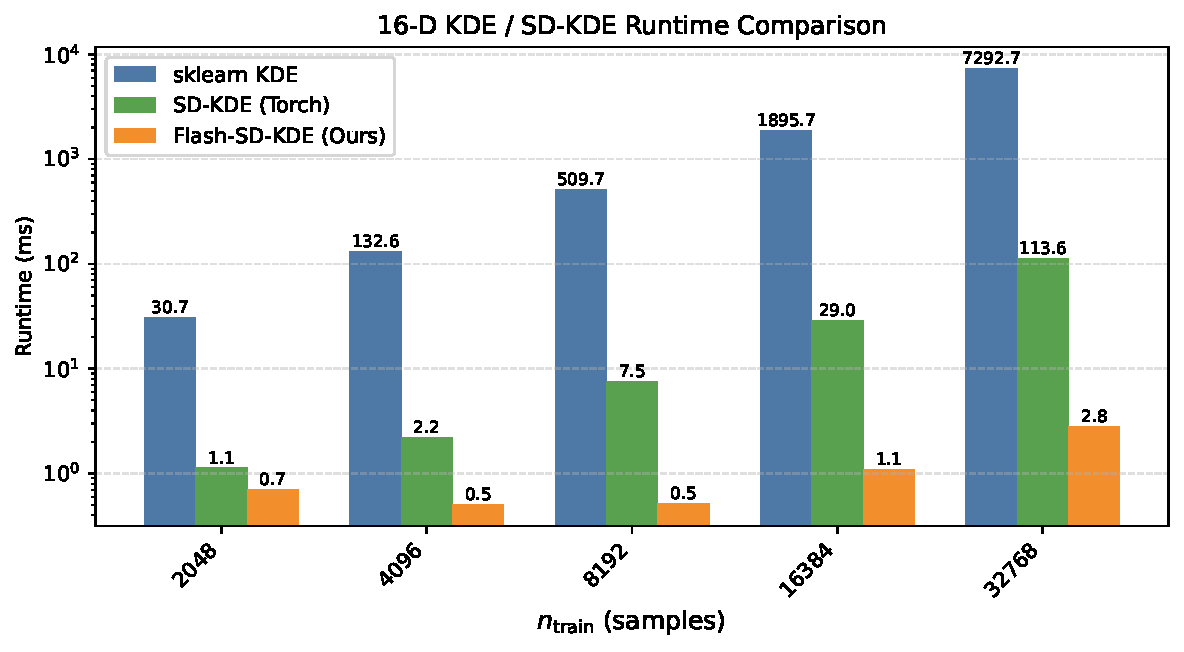
\includegraphics[width=\textwidth]{figures/runtime_16d_kde_sdkde.pdf}
  \caption{Runtime comparison for 16-D KDE/SD-KDE across $n_{\text{train}}$
           up to $32{,}768$ ($n_{\text{test}} = n_{\text{train}}/8$).}
  \label{fig:nd_runtime}
\end{figure*}
All experiments run on a workstation equipped with an NVIDIA RTX~A6000
(GA102).  This GPU exposes 84 streaming multiprocessors (SMs); each SM
contains 128 FP32 ALUs and 16 special function units (SFUs).  Because the
ratio of FP32 ALUs to SFUs is $128{:}16$, we treat one $\exp$ (issued on an
SFU) as costing the equivalent of $128/16 = 8$ FP32 flops in our models.
The card delivers roughly $40$~TFLOP/s of peak FP32 throughput and
approximately $770$~GB/s of GDDR6 bandwidth.

The host CPU is a dual-socket AMD EPYC~7763 system (``Milan'') configured
with $2 \times 64$ cores and two hardware threads per core (256 logical
CPUs reported by \texttt{lscpu}).  The processors boost up to
3.53~GHz, expose 512~MiB of shared L3 cache across the sockets, and provide
modern ISA extensions (AVX/AVX2, FMA, BMI1/2, SHA, VAES, etc.).
